\documentclass[11pt,a4paper]{article}
\usepackage[left=22mm,right=22mm,top=21mm,bottom=22mm,headheight=15pt]{geometry}
\usepackage[T1]{fontenc}
\usepackage[english]{babel}
\usepackage{tgpagella}
\usepackage[scale=.94]{tgheros}
\usepackage{inconsolata}
\usepackage{microtype}
\usepackage{graphicx,booktabs,tabularx,array,multicol}
\usepackage{amsmath,amssymb}
\usepackage{xcolor}
\usepackage{enumitem}
\usepackage{titlesec,fancyhdr,lastpage}
\usepackage{caption}
\usepackage{tikz}
\usetikzlibrary{arrows.meta,positioning}
\usepackage{hyperref}
\usepackage{bookmark}

\definecolor{ink}{HTML}{172D46}
\definecolor{teal}{HTML}{167D8D}
\definecolor{amber}{HTML}{B67518}
\definecolor{muted}{HTML}{536579}
\definecolor{light}{HTML}{EEF3F6}
\hypersetup{colorlinks=true,linkcolor=teal,urlcolor=teal,citecolor=teal,
  pdftitle={Write activity, factual access and control design in HyTorch},
  pdfauthor={Hyphae Research Foundation},
  pdfsubject={V5/V6 technical report. Measured results and a prospective protocol. English edition},
  pdfkeywords={HyTorch, factual access, experimental control, reproducibility, V5, V6}}
\urlstyle{tt}
\setlength{\parindent}{0pt}
\setlength{\parskip}{5pt}
\setlength{\emergencystretch}{1em}
\setlength{\tabcolsep}{5pt}
\renewcommand{\arraystretch}{1.16}
\setlist[itemize]{leftmargin=4.5mm,itemsep=3pt,topsep=3pt}
\setlist[enumerate]{leftmargin=6mm,itemsep=3pt,topsep=3pt}
\titleformat{\section}{\sffamily\Large\bfseries\color{ink}}{\thesection}{.65em}{}
\titleformat{\subsection}{\sffamily\normalsize\bfseries\color{ink}}{\thesubsection}{.55em}{}
\titlespacing*{\section}{0pt}{0pt}{10pt}
\titlespacing*{\subsection}{0pt}{10pt}{3pt}
\captionsetup{font=small,labelfont={bf,sf,color=ink},textfont=normalfont,skip=7pt}
\pagestyle{fancy}
\fancyhf{}
\fancyhead[L]{\sffamily\footnotesize\color{muted}HYPHAE RESEARCH FOUNDATION / HYTORCH}
\fancyhead[R]{\sffamily\footnotesize\color{muted}TECHNICAL REPORT 01}
\fancyfoot[L]{\sffamily\footnotesize\color{muted}12 September 2026 \enspace / \enspace Version 1.0 (EN)}
\fancyfoot[R]{\sffamily\footnotesize\color{muted}\thepage\ / \pageref{LastPage}}
\renewcommand{\headrulewidth}{.3pt}
\renewcommand{\footrulewidth}{0pt}
\newcommand{\sys}{\textsc{HyTorch}}
\newcommand{\status}{\texttt{no-control-match}}
\newcommand{\factloss}{\Delta_{\mathrm{Value}}}
\newcommand{\callout}[2]{\par\vspace{3pt}\begingroup\setlength{\fboxsep}{9pt}%
  \colorbox{light}{\begin{minipage}{\dimexpr\linewidth-2\fboxsep\relax}%
  {\sffamily\bfseries\color{ink}#1}\par\small #2\end{minipage}}\endgroup\par\vspace{3pt}}
\newcommand{\figurepanel}[3]{\begin{center}\includegraphics[width=\linewidth]{figures/en/#1.pdf}%
  \captionof{figure}{#2}\label{#3}\end{center}}
\newcommand{\hash}[1]{{\small\ttfamily #1}}
\newcolumntype{Y}{>{\raggedright\arraybackslash}X}
\newcommand{\pageend}{\clearpage}
\begin{document}
\thispagestyle{empty}

{\sffamily\bfseries\color{teal}\small HYPHAE RESEARCH FOUNDATION\hfill TECHNICAL REPORT 01}
\vspace{15mm}

{\sffamily\bfseries\color{ink}\fontsize{29}{34}\selectfont
Write activity,\\
factual access and\\
control design\\
in HyTorch\par}
\vspace{5mm}
{\sffamily\large\color{muted}V5 results and the prospective V6 protocol}

\vspace{6mm}
{\color{teal}\rule{\linewidth}{1.2pt}}
\vspace{2mm}

\begin{tabularx}{\linewidth}{@{}YYY@{}}
{\sffamily\bfseries\Large 2,190} & {\sffamily\bfseries\Large 50 min 46 s} & {\sffamily\bfseries\Large 2 batteries}\\[-2pt]
{\small complete measurement batches} & {\small supervised execution and closure} & {\small exact numerical agreement}\\
\end{tabularx}

\vspace{6mm}
\textbf{Summary.} A \sys{} model trained on a synthetic factual world meets the
competence criterion for common discovery facts. When writes from each of its
four units are vetoed separately, factual Value loss and original-text loss
respond differently. U0 produces the largest mean factual deterioration; U1 has
a small, heterogeneous mean factual effect despite changing control-text loss.

The complete measurement passed its integrity and repeatability checks.
However, none of the other units meets every fixed criterion for a comparable
control for U0. The final result is \status.

\callout{Conclusion and scope}{
There is evidence of a contribution to \emph{factual access} in an already
trained model. It does not yet demonstrate that a channel stops learning during
training and causes hallucinations. V6 defines a new comparison between
persistent and distributed blocking; its branches have not been trained.}

\vfill
{\small\color{muted}
A results and experimental-design document, not a research paper or a
confirmatory claim. Includes reduced data, vector figures, reconstruction code
and provenance references.\\[4pt]
Report: 12 September 2026 / Version 1.0. English edition: 13 September 2026.\\
\url{https://github.com/Hyphae-Research-Foundation/hytorch}\\[4pt]
Document, figures and data: CC BY-SA 4.0. Code: Apache-2.0.\\
Software checks and internal review; V6 has not been empirically validated.}

\pageend
\section{Question, system and scope}
\label{sec:scope}

The motivating hypothesis is that a factual function could stop improving
while other paths sustain a favorable aggregate loss. Studying this hypothesis
requires separating three claims:

\begin{enumerate}
\item An aggregate metric can conceal performance differences between functions.
\item A local failure during learning causally contributes to factual errors
and, under particular response conditions, to false assertions.
\item The mechanism is common in other models and explains a substantial share
of their hallucinations.
\end{enumerate}

This report informs the first question and prepares an intervention for the
second. It does not estimate how often the mechanism occurs in ordinary models
or its contribution to all hallucinations.

\subsection{What a unit is and what is blocked}
The model has four write sites, U0--U3, one per block. Proposals undergo
validation, allocation and quantized application to the residual. The
experimental veto converts a unit's surviving COMMITs into explicit denials,
preserving frames, original aborts and the quantization of the zero-commit
path. Losing candidates are not promoted.

An active write, a nonzero gradient or a changing codebook does not establish
factual knowledge by itself. Conversely, a small ablation effect can reflect
redundancy or variation across facts; it does not automatically identify a unit
that failed to learn.

\subsection{Task and reference}
The synthetic world assigns values to entities and relations. It distinguishes
common, rare and unexposed facts, alongside different entity-mention frequencies.
Response truth comes from the world's oracle: a chance-correct response to an
unexposed fact is still correct.

The V5 reference undergoes auxiliary warmup W640 and 4,000 acquisition updates.
It uses sequences of length 128, a vocabulary of 428 tokens and batches of 48
rows: 32 original, eight auxiliary and eight canonical. The objective combines
the three losses with weights $1$, $0.25$, $0.25$, plus global regularization
weighted by $0.001$. This recipe describes the evaluated reference; its loss
value alone does not establish its quality.

\begin{tabularx}{\linewidth}{@{}p{32mm}Y@{}}
\toprule
\textbf{Status} & \textbf{What exists at the close of this report}\\
\midrule
Observed & Reference competence and measurement of all four sites in two complete batteries.\\
Verified & Captures, reductions, records, closure and selection under the fixed rule.\\
Designed & A 17-branch V6 panel and complete schedules with mechanical tests.\\
Pending & V6 execution qualification, branch training and causal results.\\
\bottomrule
\end{tabularx}

\pageend
\section{Factual competence of the reference}
\label{sec:competence}

The reference passes the \emph{common-discovery} competence gate: at least 80\%
macro accuracy and strict superiority over all four declared priors in each
position map. This result concerns the common-fact subset. Performance on the
complete population is substantially lower.

\figurepanel{competence}{Reference accuracy by stratum and position map. Each
series retains its denominator. Common-fact accuracy is not accuracy over all
128 questions. No confidence intervals are shown: maps and questions are not
independent training replicates.}{fig:competence}

\begin{tabularx}{\linewidth}{@{}Yrrrr@{}}
\toprule
\textbf{Map} & \textbf{Common} & \textbf{Rare} & \textbf{Unexposed} & \textbf{Overall}\\
\midrule
Identity & 38/38 & 26/38 & 3/52 & 67/128\\
Shift 8 & 36/38 & 30/38 & 4/52 & 70/128\\
Gaps 4 & 37/38 & 23/38 & 3/52 & 63/128\\
\bottomrule
\end{tabularx}

The evaluation covers 64 discovery facts with two questions per fact: 19
common, 19 rare and 26 unexposed. Overall accuracies are 52.34\%, 54.69\% and
49.22\%. Common-fact accuracies are 100\%, 94.74\% and 97.37\%. The four common
priors achieve 0\%, 5.263\%, 10.526\% and 10.526\%.

All 384 responses are present. Coverage is 100\%, with no abstentions or invalid
outputs; errors are false assertions in this benchmark. These results belong
to the already trained reference and do not compare causal blocking or rescue
training branches.

\callout{Sufficient competence within a limited scope}{
The reference supports a study of access contributions for common facts the
system can answer. It does not establish uniform knowledge of rare or unexposed
facts, or general language capability.}

\pageend
\section{How the measurement was performed}
\label{sec:method}

The A4000 reference was frozen and two batteries were run with membership,
order and rules fixed in advance. Each input was evaluated without a veto and
with each of the four singleton vetoes. This phase involved no parameter
updates or training.

\begin{center}
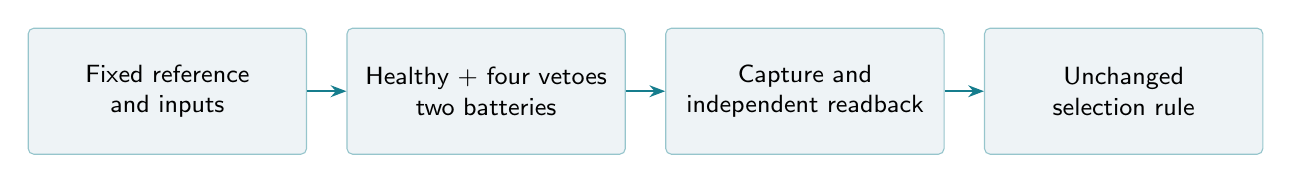
\begin{tikzpicture}[node distance=5mm,box/.style={draw=teal!45,fill=light,rounded corners=2pt,
  text width=33mm,minimum height=16mm,align=center,font=\sffamily\small},
  arr/.style={-{Stealth[length=2mm]},draw=teal,thick}]
\node[box] (a) {Fixed reference\\and inputs};
\node[box,right=of a] (b) {Healthy + four vetoes\\two batteries};
\node[box,right=of b] (c) {Capture and\\independent readback};
\node[box,right=of c] (d) {Unchanged\\selection rule};
\draw[arr] (a)--(b);\draw[arr] (b)--(c);\draw[arr] (c)--(d);
\end{tikzpicture}
\end{center}

\subsection{Factual localization}
Factual loss is measured at the public answer boundary, before supplying the
correct Value token. It uses the full distribution over 428 classes, without
renormalizing over the possible values:
\begin{align}
\ell_{f,q,p}^{(u)}&=-\log\operatorname{softmax}(z_{f,q,p}^{(u)})[v_f],\\
\factloss(u)&=\frac{1}{|F|}\sum_{f\in F}
  \frac{1}{|Q_f||P|}\sum_{q\in Q_f,p\in P}
  \left(\ell_{f,q,p}^{(u)}-\ell_{f,q,p}^{(\varnothing)}\right).
\end{align}
Each fact receives equal weight, after averaging its questions and positions.
A positive value means that vetoing the unit reduces the geometric mean
probability assigned to the correct Value. Nats are not accuracy percentage points.

\subsection{Measuring general disruption}
The inventory contains all 1,120 original text occurrences for discovery
entities, preserving multiplicities, the factual/mention mixture, valid targets
and EOS. NLL is token-weighted within each map, and the three maps receive equal
weight. The following quantities are retained for each unit:
\begin{tabularx}{\linewidth}{@{}p{15mm}Y@{}}
\toprule
$g_u$ & Signed change in original-text NLL: veto minus healthy.\\
$m_u$ & RMS of the difference between the ordinary local write output and the quantized zero-commit output.\\
$r_u$ & RMS of that local zero-commit output; $\rho_u=m_u/r_u$.\\
$p_u$ & Admitted candidates among all valid candidates on the healthy path, including overflows and aborts in the denominator.\\
\bottomrule
\end{tabularx}

RMS values are computed from global sums of squares and counts, not by
averaging batch RMS values. The proxy $g$ uses known text from this task; it
does not measure functional equivalence between units or disruption of language
as a whole.

The complete population comprises 219 input sets, 2,190 batches, 34,740 real
coordinates and 300 dummy rows excluded from metrics. Facts were not filtered
according to the reference's correct answers.

\pageend
\section{Contributions of the four units}
\label{sec:units}

U0 leads the localizer in both batteries: $\factloss=0.880215$ nats, with a gap
of $0.241685$ over U2. U2 and U3 also have positive mean factual effects.
The observed contribution is not exclusive to U0.

\figurepanel{channel-effects}{Factual and original-text effects, with their scales
and position-specific breakdowns. The metrics use different populations and
denominators. Both batteries produce the same values; drawing two copies would
not add an independent replicate.}{fig:units}

\begin{tabularx}{\linewidth}{@{}Yrrrrrr@{}}
\toprule
\textbf{Unit} & $\factloss$ & $g$ & $m$ & $r$ & $\rho$ & $p$\\
\midrule
U0 & 0.880215 & 0.114421 & 0.533184 & 1.178609 & 0.452384 & 0.641188\\
U1 & $-0.021274$ & 0.142184 & 0.528574 & 1.293221 & 0.408727 & 0.637110\\
U2 & 0.638529 & 0.042236 & 0.541165 & 1.417010 & 0.381906 & 0.674473\\
U3 & 0.504185 & 0.030009 & 0.540632 & 1.529304 & 0.353515 & 0.658546\\
\bottomrule
\end{tabularx}
{\footnotesize Values are rounded for readability. Both complete batteries and
full-precision values are included in the report data.}

U1 has a small, slightly negative mean factual effect alongside a larger increase
in original-text NLL than U0. This aggregate difference is informative but depends
on the facts and maps evaluated. Its writes are active: the result does not
identify a dead channel or a module dedicated exclusively to general language.

\pageend
\section{Why no matched control was obtained}
\label{sec:matching}

The rule required a factual effect greater than $0.05$ nats in both batteries,
stable selection and a control distinct from the target satisfying four
criteria. For the leading unit U0, the text-loss margin is:
\[
s_g=\max(0.02,\ 0.20|g_{U0}|)=0.0228841794.
\]
A candidate therefore needed $g$ within
$[0.091536718,\ 0.137305076]$.

\figurepanel{matching}{Candidate evaluation under the fixed limits. The band is
an admissibility criterion, not a confidence interval. All three candidates
fail the text-NLL criterion and pass the other three.}{fig:matching}

\begin{tabularx}{\linewidth}{@{}Yrrrr@{}}
\toprule
\textbf{Candidate} & $|g_u-g_{U0}|$ & $m_u/m_{U0}$ & $\rho_u/\rho_{U0}$ & $|p_u-p_{U0}|$\\
\midrule
U1 & 0.027763 & 0.991354 & 0.903495 & 0.004078\\
U2 & 0.072185 & 1.014968 & 0.844207 & 0.033285\\
U3 & 0.084411 & 1.013968 & 0.781448 & 0.017358\\
\midrule
Limit & $\leq0.022884$ & $[2/3,1.5]$ & $[2/3,1.5]$ & $\leq0.10$\\
\bottomrule
\end{tabularx}

U1 is the closest candidate but still exceeds the NLL limit by $0.004878687$
nats. The result does not depend on rounding: the decision uses full-precision
values. Calipers were not widened, the target was not replaced, and no additional
batteries were added to obtain a favorable result.

\textbf{Final result: \status.} The final target and control identifiers are
null. U0 remains the localizer leader; the original matched comparison is not
admitted.

\pageend
\section{Heterogeneity: the mean does not describe every fact}
\label{sec:heterogeneity}

The per-fact breakdown retains information lost in a single bar. All 19 of
U0's mean per-fact effects are positive, but their magnitudes vary. For U1,
eight facts have positive effects and eleven have negative effects, ranging
approximately from $-0.249738$ to $0.237074$ nats.

\figurepanel{fact-heterogeneity}{Factual effect by fact and unit, averaged over two
questions and three maps. All 19 facts and a zero-centered scale are retained.
Values are rounded: very small values may appear as zero. Cells are not
independent training replicates.}{fig:heterogeneity}

\begin{tabularx}{\linewidth}{@{}Yrrrr@{}}
\toprule
\textbf{Map} & $\factloss(U0)$ & $\factloss(U1)$ & $g_{U0}$ & $g_{U1}$\\
\midrule
Identity & 1.194326 & $-0.050548$ & 0.148076 & 0.050147\\
Shift 8 & 0.652737 & $-0.024324$ & 0.119203 & 0.172679\\
Gaps 4 & 0.793581 & 0.011050 & 0.075983 & 0.203725\\
\bottomrule
\end{tabularx}

U1's larger average text disruption relative to U0 does not occur in the
identity map: it appears under the position transformations. The sign of U1's
factual effect also varies across maps. The aggregate result therefore does
not establish a simple division between a ``facts'' unit and a ``language'' unit.

This heterogeneity does not by itself explain a persistent learning failure.
That hypothesis requires comparing intervened training trajectories with their
controls.

\pageend
\section{Integrity, repeatability and interpretation limits}
\label{sec:integrity}

The measurement closed in 3,046.425 seconds, within the authorized 90 minutes,
without an automatic restart. The supervisor recorded return code zero, an
empty process group and confirmed closure. The final result was no longer
provisional before the tables in this report were produced.

\begin{tabularx}{\linewidth}{@{}p{47mm}Y@{}}
\toprule
\textbf{Check} & \textbf{Result and scope}\\
\midrule
Complete capture & 2,190 batches and both batteries; no coordinates omitted to improve selection.\\
Independent readback & 19,656,415,525 bytes read; numerical reductions and tables reconstructed from the captures.\\
Native records & 2,193 ordered records checked: run startup and start, batch and end commitments. Query performed on a fresh copy of the stopped ledger.\\
Final custody & Namespace and metadata continuity for 39,722 files in 4,383 directories.\\
Repetition & Maximum NLL and RMS drift: zero; integer classification counts identical.\\
Selection & Complete rule and membership recomputed; \status\ at closure.\\
\bottomrule
\end{tabularx}

\subsection{What these checks establish}
Raw readback checks its reductions; Native links records and receipts but does
not itself determine factual truth or authenticate all neural arithmetic. The
final custody check preserves continuity of previously hashed files on a trusted
filesystem; it does not guarantee protection against adversarial rewrites that
preserve metadata. The checks have complementary scopes.

The B16 path was qualified against the reference and sham at the same geometry.
Changing from B1 to B16 is not bit-identical for every logit, although no greedy
decision changed in the fixed diagnostic. Those identities and limits remain
recorded; CPU qualification does not extend to GPU or XLA. The cited competence
evaluation comes from a completed recovery; prior operational failures remain
in the historical provenance.

\subsection{What has not been demonstrated}
\begin{itemize}
\item The two batteries repeat the same population numerically; they are not
two independent seeds or worlds and do not establish statistical significance.
\item Ablating a trained model measures access/prediction. It does not show
that facts were never acquired or that a path stores them exclusively.
\item An NLL measurement is not a classification of a generated response as
a hallucination. The channel measurement did not run H/T/C/R training branches.
\item An active local contribution or an active aggregate gradient does not
prove factual learning by an individual unit. U1's small mean effect does not
prove channel death either.
\end{itemize}

\callout{A useful finding; the causal hypothesis remains open}{
The evidence links an access intervention to measurable changes in factual
probability and documents the limit of the original control. The relationship
between channel death during learning and false assertions remains unproven.}

\pageend
\section{V6: persistent and distributed blocking}
\label{sec:v6}

The new protocol preserves \status\ and explicitly changes the estimand.
It compares persistent/concentrated blocking policies with distributed
interruptions, balancing site and input marginals at every update of the panel.
It does not manufacture a match for U0 or assume equal general damage along
the training trajectories.

\figurepanel{prospective-design}{Schedules derived from the fixed V6 plan.
\textbf{This is a prospective design: the branches have not been trained.}
Colors identify the site scheduled for a veto; they are not measured losses or
outcomes. Rescue branches remove the block from update index 2000.}{fig:v6}

The panel has 17 branches: a healthy sham H, four P branches with one fixed unit
blocked, four D branches with distributed blocks and eight RP/RD rescue branches.
All start from the same A0 within the world/seed and finish at A4000 with the
same examples and horizon.

For $b=\lfloor t/4\rfloor$, $k=t\bmod4$ and a permutation $\pi_b$ fixed by
hashing an independent seed, without consuming model or data RNG state, D$_s$
vetoes $\pi_b[(k+s)\bmod4]$. Each set of four P or D branches assigns each site
exactly once per update. Each D visits all sites once per four-update block;
it is not permanently tied to the same auxiliary slice of the curriculum.

Each P concentrates 4,000 scheduled blocks in one site; each D distributes
1,000 per site. This balance does not equalize effective COMMITs, removed energy
or gradients once parameters diverge. RP/RD match their P/D counterparts through
A2000 and use sham from update index 2000, which produces A2001. Primary
inference is unblocked. Each branch is executed as a separate complete run;
strict resume does not permit switching schedules.

\pageend
\section{What V6 will estimate and what execution requires}
\label{sec:future}

For each final outcome $Y$, bars denote the mean over the four branches in each
family:
\begin{align*}
\tau&=\overline{Y}_P-\overline{Y}_D, &
\rho_P&=\overline{Y}_{RP}-\overline{Y}_P,\\
\rho_D&=\overline{Y}_{RD}-\overline{Y}_D, &
\kappa&=\rho_P-\rho_D.
\end{align*}
$\tau$ is the total policy contrast. $\kappa$ measures how that difference
changes when both types of block are removed. H contextualizes competence and
damage; effects at different sites need not be assumed additive.

\subsection{Outcomes, data and limits}
The protocol fixes a new realization of the world, exposure, model and
schedule. The unit of replication is the world/seed, not the 17 branches, facts
or positions. All failures are retained, and seeds are not replaced after
unfavorable results.

Primary evaluation uses all common validation facts at A4000, including those
H answers incorrectly; rare and unexposed strata are also reported. Factual
metrics average by fact. Original-text NLL uses a separate global inventory:
all original TRAIN occurrences for validation entities, weighted by valid
tokens/EOS within each map. Their denominators are not mixed.

All 17 training runs close and are verified before validation capture. Public
generations and full answer-boundary logits, without the correct Value in the
input, are sealed first; private targets partitioned by split are opened only
afterward. The historical reader that loads a combined oracle requires a
qualified replacement. Validation in the old world was already evaluated in
V2: it is not globally blind merely because V5 did not read it. Test remains
closed in the new protocol.

A descriptive margin of 0.02 nats is fixed for jointly interpreting original-text
NLL and factual deterioration by map. It is neither a functional-equivalence
test nor a gate for excluding, reweighting or rerunning branches after observing
them. Curves and access diagnostics are fixed in advance. A finite rescue can
combine restored access with additional learning; it does not automatically
identify a unique mechanism, and failure does not prove irreversibility.

\subsection{Resources and technical preparation}
\begin{tabularx}{\linewidth}{@{}Y>{\raggedright\arraybackslash}p{48mm}@{}}
\toprule
\textbf{Item} & \textbf{Historical serial CPU base}\\
\midrule
17 acquisition runs & 39 h 2 min (approx.)\\
17 branches with verification, three maps and postrun & 56 h 18 min 50 s\\
New W640 and shared initialization & +14 min 30 s (approx.)\\
Full pre/post example only & 398.4375 GiB for 17 branches\\
\bottomrule
\end{tabularx}

These figures extrapolate from historical terminal records; they are not a
sufficient cap for the new runner. They exclude qualification, new curves,
diagnostics, other captures, copies and contingency. No parallel speedup or
shared-prefix savings are assumed. GPU/AMD requires its own qualification and
measured costs.

The schedule passed 62 tests and the package passed six additional checks.
That validates pure design components. The new schedule family in the kernel,
guard and Native, the export and private reader, qualified initialization and
numerical execution, and the full budget remain pending. No V6 training has
been performed.

\pageend
\section{Reproducibility and provenance}
\label{sec:provenance}

This report includes LaTeX source, five vector figures, reduced data and
reconstruction scripts. A clean clone can rebuild the figures and recompute
selection without loading a model, querying Native or downloading the complete
raw captures.

\begin{tabularx}{\linewidth}{@{}>{\raggedright\arraybackslash}p{43mm}Y@{}}
\toprule
\textbf{Included artifact} & \textbf{What it supports checking}\\
\midrule
\texttt{data/report-data.json} & Curated competence, unit, position and fact data, limits and the illustrated schedule.\\
\texttt{data/provenance.json} & Original sources, extraction fields and hashes; originals distinguished from reduced exports.\\
Tables and selector in \texttt{data/} & Recompute both batteries' aggregates and decision under the original rule from their complete tables.\\
\texttt{design/} & V6 protocol, complete schedule and pure balance verification.\\
\texttt{make\_figures.py} & Rebuild localized figures from portable data; no post hoc example selection.\\
\texttt{report-en.tex}, \texttt{Makefile} & Compile the English technical PDF; no experimental execution.\\
\bottomrule
\end{tabularx}

Reproducing tables and figures does not replace full revalidation from the
original raw files, checkpoints and ledgers, which are not included. The
historical readback counter recorded approximately 19.66 GB read; it is not
the combined size of those three evidence types. The exporter authenticates
the pinned source JSON and documents when available, without revalidating raw
blobs or checkpoints. This package neither reconstructs the historical training
trajectory nor qualifies a future run merely by containing its hashes.

\subsection{Principal identifiers}
Repository-relative paths and the complete source list are in the provenance
manifest. The following SHA256 hashes identify cited closures and rules. The
V6 protocol hash is for the frozen Spanish source, not its English translation.

{\footnotesize
\begin{tabularx}{\linewidth}{@{}p{32mm}Y@{}}
\toprule
\textbf{Evidence} & \textbf{SHA256 of the original artifact}\\
\midrule
V5 competence & \texttt{bdb63840ae28176e5cbf22aded90ad78585804415e0d5579ca9bb63da1bee9db}\\
Worker closure & \texttt{f223ec5ec1101a67528a4cd54d38ce9e4d7dd405ad0c26586f63c360d42810a2}\\
Supervisor closure & \texttt{18b41a1980e6eef486a1747789cbb04b06154f403da7d52de9780a968acc6002}\\
V5 selection & \texttt{ef1b3cbb783364b662974c0a605b42a9758433b2b77c864a644d08f1d6bfa78f}\\
V1 rule & \texttt{a9f1aef9f00e5bb98aa7fe9e294771f279c0693a9815ae40a1ea34167d469f79}\\
V6 protocol (ES) & \texttt{6bae2857c9bf6910aa728be2cd65da5f510400190f2e45a1d909194bd48ea195}\\
V6 plan file & \texttt{feb9d0cbb236831a864a4f8981772262953f198fa53570ecde01b3704c95f766}\\
\bottomrule
\end{tabularx}}

The frozen causal source used for measurement corresponds to commit:
\begin{center}\texttt{033450e50d6a13b355b010cabaacf686a741d25f}\end{center}
Its identity remains distinct from the historical reference's source identity.
No hash in this report confers scientific admission or training authorization.

\subsection{Closing interpretation}
The results justify measuring factual contributions alongside activity and
aggregate loss. They also document a real limit of the initial design: none of
the three candidates is an admissible control under the fixed rule. V6 proposes
a different, explicit comparison for studying persistent blocking. The causal
hypothesis remains open until that study is executed and evaluated within its
declared scope.

\end{document}
